% !TEX program = xelatex
\documentclass[usenames,dvipsnames]{beamer}
\usefonttheme{serif}
\usefonttheme{structuresmallcapsserif}
\usetheme{Copenhagen}
\usepackage{xcolor}
\beamertemplatenavigationsymbolsempty
\usepackage{tikz}
% \usepackage{pgfplots}
\renewcommand{\qed}{\hfill\blacksquare}
\newcommand{\D}[1]{\Delta #1}
\renewcommand{\a}{\alpha}
\usepackage{float}
\usepackage{pgfplots}
\pgfplotsset{compat = newest}
\usetikzlibrary{positioning, arrows.meta}
\usepgfplotslibrary{fillbetween}
\usepackage{amsmath ,amssymb,amsthm}
\setbeamertemplate{frametitle continuation}{%
    \ifnum\insertcontinuationcount>999999999 % this command tells the program when to start counting and also the count will be in numbers and not in roman letters
    \insertcontinuationcount
    \fi}
% ============================================================ %
% HEBREW support via polyglossia %
% ============================================================ %
\usepackage{polyglossia}
\defaultfontfeatures{Mapping=tex-text, Scale=MatchLowercase}
\setdefaultlanguage{hebrew}
\setotherlanguage{english}
\newfontfamily\hebrewfont[Script=Hebrew]{Arial}
% Use \begin{hebrew} block of text \end{hebrew} for paragraphs.
% Use \texthebrew{ } and \textenglish{ } for short texts.
% ============================================================ %
\title{תרגול 8 - השקעות ב' - שוק הדיור}
\author{\texthebrew{ מתן לבינטוב}}
\institute[{{ אב"ג}}]{{ אוניברסיטת בן גוריון בנגב}}
\date{12 לדצמבר 2023}
\usepackage{bidi}
\begin{document}
\begin{RTL}
\begin{frame}
\titlepage
\end{frame}

\begin{frame}
    \frametitle{נושאים}
    \tableofcontents
\end{frame}

\section{השקעות בדיור}
\begin{frame}[allowframebreaks]
    \frametitle{השקעות בדיור}
המודל מחולק ל4 חלקים: 
\begin{enumerate}
    \item שוק השכירות
    \item שוק הדירות
    \item היצע הקבלנים
    \item הצבר הון בסוף תקופה
\end{enumerate}
    
\framebreak

\begin{block}{1. שוק השכירות}
    בשוק זה נקבע שכר הדירה, הוא נקבע לפי היצע הדירות בשוק ולפי הביקוש לדירות
    $$ H^d \downarrow \implies R \downarrow $$
    $$ H^d \uparrow \implies R \uparrow $$
\end{block}
\framebreak
\begin{block}{2. שוק הדירות}
    התשואה על דירה הינה :
    $$ RR = \frac{R - D }{P_H} + \frac{P_H^{e}}{P_H} $$
    כל עוד התשואה על דירה גדולה יותר מהריבית על חיסכון, עדיף להשקיע בדירה ולהפך, כלומר בש''מ ($RR = r$)
    \\
     בנוסף נניח שאין ציפיות לשינוי מחיר הדירה ($P_h^e = 0 $)
    לכן ,
    $$P_H = \frac{R}{r+d}$$
\end{block}
\framebreak
\begin{block}{3. היצע הקבלנים}
    קבלני הדירות מספקים את היצע הדירות ככל שמחיר הדירה גבוה יותר כך הם בונים יותר דירות.
    \\
    פונקצית ההיצע שלהם תהיה :
    $$P_h = mc $$

    במילים, הקבלנים בונים עד שמחיר הדירה שווה למחיר הבנייה השולית של הדירה.
    
\end{block}

\framebreak
\begin{block}{4. הצבר הון בסוף תקופה}
    בסוף תקופה בודקים כמה דירות חדשות נבנו וכמה דירות נהרסו, \\ 
    כאשר מסמנים את $q$ בתור מספר הדירות החדשות שנבנו בתקופה.\\
    ואת $d$ כאחוז הדירות שנהרסו בסוף תקופה ולכן $d \cdot H^s$ הינו מספר הדירות שנהרסו בתקופה.
    $$\begin{cases}
        q - d \cdot H^s > 0 \implies \uparrow H^s \\
        q - d \cdot H^s < 0 \implies \downarrow H^s   
    \end{cases}$$
    אם כמות הדירות שנבנו שווה לכמות הדירות שנהרסו, $q = d\cdot H^s$ אזי אנחנו בהיצע דירות יציב ואנחנו קוראים לנקודה הזאת טווח ארוך
\end{block}

\framebreak
\begin{figure}
    \begin{small}
        \begin{center}
            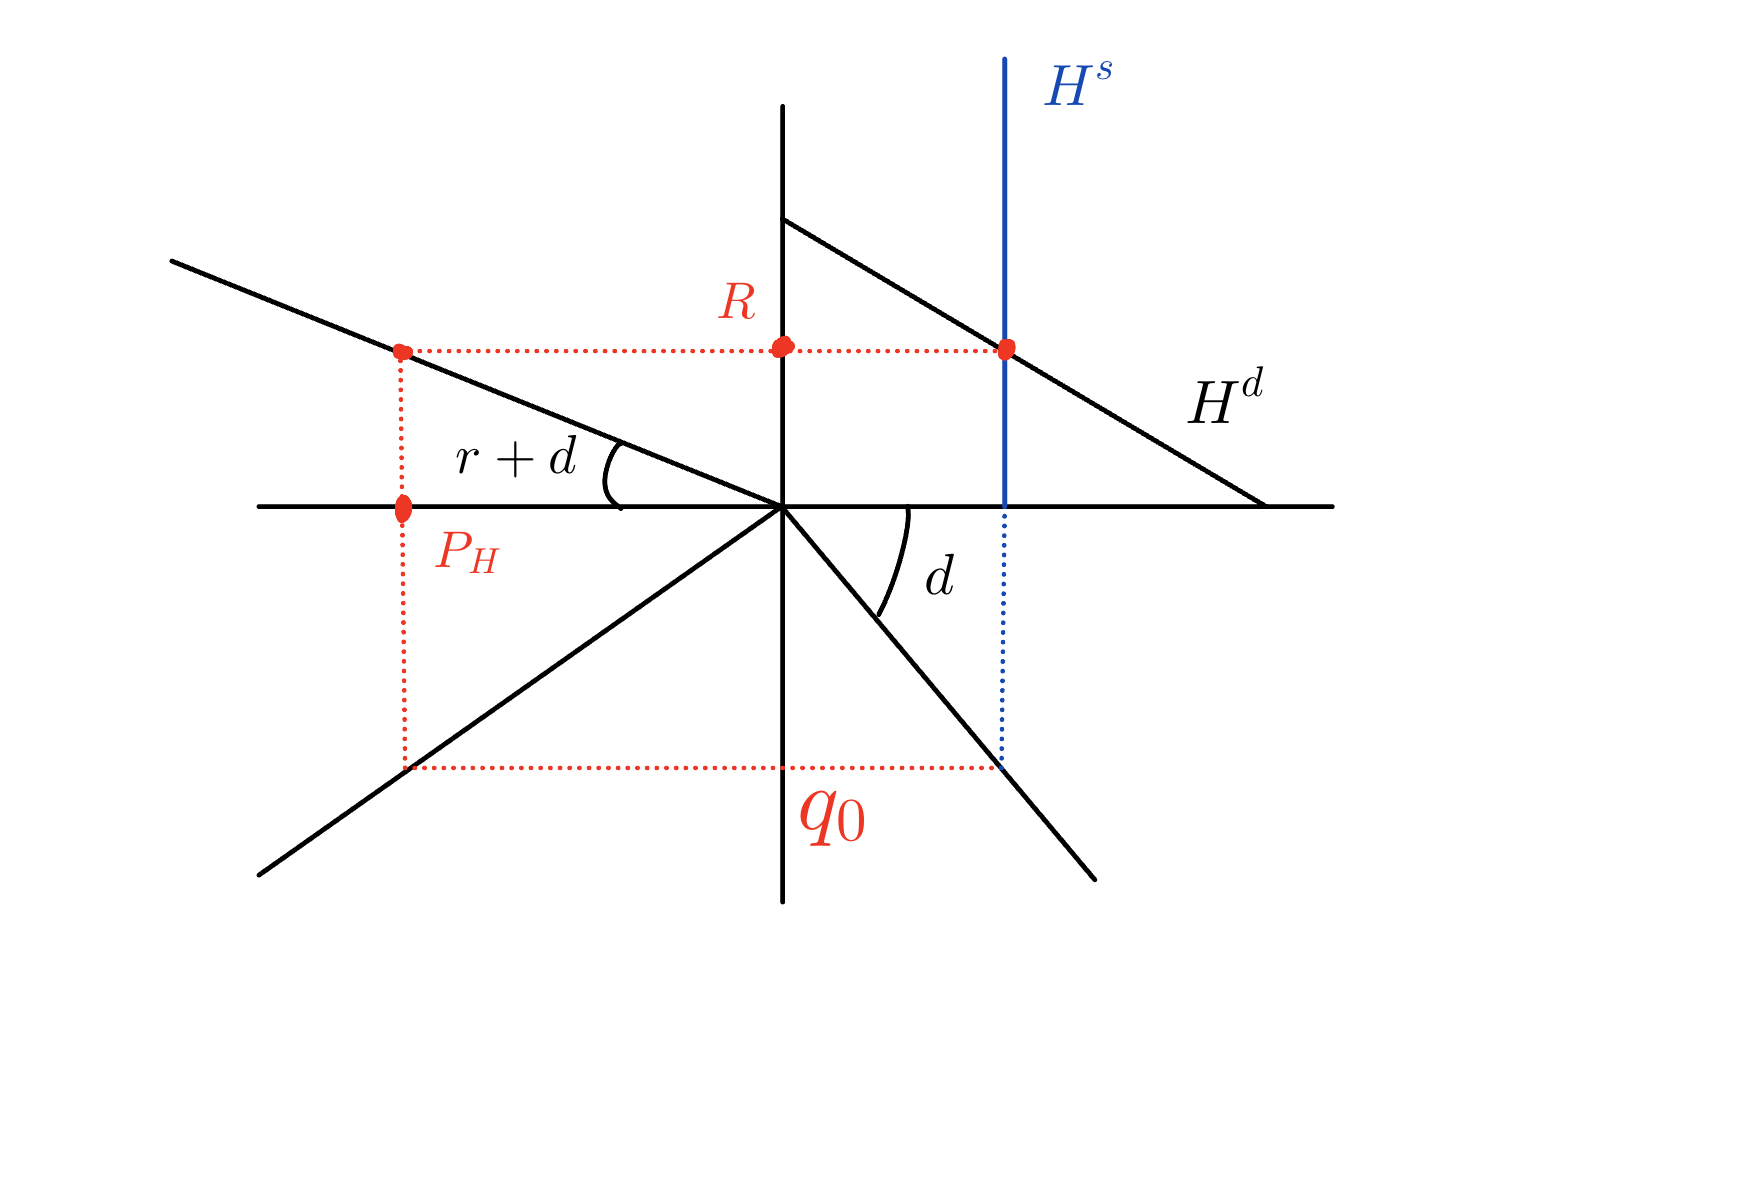
\includegraphics[width=1.2\textwidth]{figures/SCR-20231209-nblm.png}
        \end{center}
        % \caption{}
        % \label{fig:}
    \end{small}
\end{figure}


\framebreak
\begin{block}{שיטת פיתרון}
    הולכים נגד כיוון השעון, מתחילים ברביע הראשון ואז הולכים שמאלה, ואז למטה ואז ימינהו אז חוזרים לרביע הראשון.
    \\
    בכל ש''מ מתקיים :
    $$\begin{cases}
        P_H = mc \\ 
        P_H = \frac{R}{r+d}\\ 
        H^D = H^S
    \end{cases}$$
\end{block}
\end{frame}



\section{תזכורת קצרה לגבי גמישויות}
\begin{frame}[allowframebreaks]
    \frametitle{תזכורת קצרה לגבי גמישויות}

    

\end{frame}
\end{RTL}
\end{document}